%%%% ijcai22.tex

\typeout{Offline Time-Independent Multi-Agent Path Planning}

% These are the instructions for authors for IJCAI-22.

\documentclass{article}
\pdfpagewidth=8.5in
\pdfpageheight=11in
% The file ijcai22.sty is NOT the same as previous years'
\usepackage{ijcai22}

% Use the postscript times font!
\usepackage{times}
\usepackage{soul}
\usepackage{url}
\usepackage[hidelinks]{hyperref}
\usepackage[utf8]{inputenc}
\usepackage[small]{caption}
\usepackage{graphicx}
\usepackage{amsmath}
\usepackage{amsthm}
\usepackage{amssymb}
\usepackage{booktabs}
\usepackage{algorithm}
\usepackage{algpseudocode}
\usepackage{multirow}
\usepackage[export]{adjustbox}
\urlstyle{same}
\usepackage[binary-units]{siunitx}

\usepackage{tikz}
\usetikzlibrary{calc}
\usetikzlibrary{positioning}
\usetikzlibrary{shapes.geometric}
\usetikzlibrary{patterns}
\tikzset{
vertex/.style={circle,draw,black,align=center,inner sep=0cm, minimum size=0.5cm,fill=white,anchor=center},
agent/.style={vertex,fill={rgb:red,1;green,1;blue,1},text=white},
agent1/.style={agent,fill={rgb:red,0;green,1;blue,3}},
agent2/.style={agent,fill={rgb:red,3;green,1;blue,0}},
agent3/.style={agent,fill={rgb:red,1;green,3;blue,2}},
line/.style={black}
}
\usepackage[font=small,subrefformat=parens]{subcaption}
%
\usepackage{macro}

% the following package is optional:
%\usepackage{latexsym}

% See https://www.overleaf.com/learn/latex/theorems_and_proofs
% for a nice explanation of how to define new theorems, but keep
% in mind that the amsthm package is already included in this
% template and that you must *not* alter the styling.
\newtheorem{theorem}{Theorem}[section]
\newtheorem{lemma}[theorem]{Lemma}
\newtheorem{proposition}[theorem]{Proposition}
\newtheorem{corollary}[theorem]{Corollary}
\newtheorem{observation}[theorem]{Observation}
\newtheorem{definition}[theorem]{Definition}
\newenvironment{sketch}{\renewcommand{\proofname}{Proof sketch}\proof}{\endproof}
\newtheorem*{theorem*}{Theorem}
\newtheorem*{lemma*}{Lemma}
\newtheorem*{proposition*}{Proposition}

\usepackage{multibib}
\newcites{Appendix}{Additional References}

% Following comment is from ijcai97-submit.tex:
% The preparation of these files was supported by Schlumberger Palo Alto
% Research, AT\&T Bell Laboratories, and Morgan Kaufmann Publishers.
% Shirley Jowell, of Morgan Kaufmann Publishers, and Peter F.
% Patel-Schneider, of AT\&T Bell Laboratories collaborated on their
% preparation.

% These instructions can be modified and used in other conferences as long
% as credit to the authors and supporting agencies is retained, this notice
% is not changed, and further modification or reuse is not restricted.
% Neither Shirley Jowell nor Peter F. Patel-Schneider can be listed as
% contacts for providing assistance without their prior permission.

% To use for other conferences, change references to files and the
% conference appropriate and use other authors, contacts, publishers, and
% organizations.
% Also change the deadline and address for returning papers and the length and
% page charge instructions.
% Put where the files are available in the appropriate places.

% PDF Info Is REQUIRED.
% Please **do not** include Title and Author information
\pdfinfo{
/TemplateVersion (IJCAI.2022.0)
}

\title{Offline Time-Independent Multi-Agent Path Planning}

% Single author syntax
\author{
  Keisuke Okmura\footnote{Contact Author}\and
  Fran\c{c}ois Bonnet\and
  Yasumasa Tamura\And
  Xavier D\'{e}fago\\
  \affiliations
  Tokyo Institute of Technology\\
  \emails
  \{okumura.k, bonnet.f, tamura.y, defago.x\}@coord.c.titech.ac.jp
}

\begin{document}

\maketitle
\begin{abstract}
This work presents an optimization method for generating kinodynamically feasible and collision-free multi-robot trajectories that exploits an incremental denoising scheme in diffusion models. Our key insight is that high-quality trajectories can be discovered merely by denoising noisy trajectories sampled from a distribution. This approach has no learning component, relying instead on only two ingredients: a dynamical model of the robots to obtain feasible trajectories via rollout, and a fitness function to guide denoising with Monte Carlo gradient approximation. The proposed framework iteratively optimizes a deformation for the previous trajectory with the current denoising process, allows \textit{anytime} refinement as time permits, supports different dynamics, and benefits from GPU acceleration. Our evaluations for differential-drive and holonomic teams with up to 16 robots in 2D and 3D worlds show its ability to discover high-quality solutions faster than other black-box optimization methods such as MPPI. In a 2D holonomic case with 16 robots, it is almost twice as fast. As evidence for feasibility, we demonstrate zero-shot deployment of the planned trajectories on eight multirotors.
\end{abstract}

\section{Introduction}
The eventual goal of collective path planning for multiple agents is to make each agent in a shared workspace be on their respective goal status.
This problem becomes non-trivial when agents cannot pass through each other, i.e., each agent occupies some resources in the space while the others are blocked to access these resources at that time.
We see such situations in fleet operations of warehouses~\cite{wurman2008coordinating}, intersection management for self-driving cars~\cite{dresner2008multiagent}, multi-robot 3D printing systems~\cite{zhang2018large}, packet-switched networks with limited buffer spaces~\cite{tel2000introduction}, and lock operations of transactions on distributed databases~\cite{knapp1987deadlock}, to name just a few.

In such multi-agent systems, each agent inherently takes and finishes actions (or moves) \emph{at their own timings independently and unpredictably from other actors}, regardless of centralized or decentralized controls.
This is due to the nature of \emph{distributed environments} such as message delay or clock shift/drift, as well as uncaptured individual differences between agents like frictions of physical robots.
Nevertheless, the cutting‐edge research on pathfinding for multiple agents, known as Multi-Agent Path Finding (MAPF)~\cite{stern2019def} that aims at finding a set of collision-free paths on graphs, heavily rely on timing assumptions.
Typical MAPF assumes that agents take actions just at the same time.
Not to mention, such ``timed'' schedules contradict the nature of distributed environments.
Even worse, on-time execution of offline planning is too optimistic with more agents.

One counter approach to the timing uncertainties is runtime supports by online monitoring, re-planning, and intervention, e.g.,~\cite{van2011reciprocal,ma2017multi,atzmon2020robust,okumura2021time}.
This approach however requires runtime effort and additional infrastructures (e.g., steady network and monitoring systems) to manage agents' status in real-time.
Moreover, how to realize such schemes in large systems is not trivial at all.

Instead, this paper studies a novel planning problem in which agents spontaneously take actions without any timing assumptions. The problem requests a set of paths (i.e., solution) ensuring that all agents eventually reach their destinations without blocking each other permanently.
To see this, consider the situation in Fig.~\ref{fig:example}(left).
This plan runs a risk of execution failure;
if the agent $j$ gets delayed for any reason while the agent $i$ moves two steps to the right, then each agent blocks each other and neither agent can progress on its respective path.
In contrast, in Fig.~\ref{fig:example}(right), regardless of how the two agents are scheduled, both agents eventually reach their destinations unless they permanently stop the progression.
We call the corresponding problem \emph{Offline Time-Independent Multi-Agent Path Planning (OTIMAPP)}.

A special case of the error reconstruction problem is that of localizing a multi-agent system using inter-agent measurements, which has been previously studied using \textit{rigidity theory} \cite{zhao2019bearing}. In this subsection, we consider the specific example of multi-agent localization using inter-agent distances, using it to illustrate the relevance of Theorem \ref{thm:generalized}, as well as motivate our forthcoming analysis. 

Consider the example where $\mathbf p[i]\in \mathbb R^3$ is the $i^{th}$ agent's position vector and each component of $\mathbf \Phi$ is of the form
\begin{equation}
    \mathbf \Phi^{(l)}(\mathbf p)=\|\mathbf p[i] - \mathbf p[j]\|
\end{equation}
where $\mathcal E^{(l)}=\lbrace i, j\rbrace$. This gives us the dimensions $n=3|\mathcal V|$ and $m=|\mathcal E|$ of the domain and codomain of $\mathbf \Phi$, respectively. In this case, the matrix $\mathbf J_{\mathbf \Phi}(\mathbf p)\in \mathbb R^{|\mathcal E|\times 3|\mathcal V|}$ is called the \textit{rigidity matrix}, and its maximal rank is well-known to be equal to $(3|\mathcal V|-6)$ \cite{eren2004rigidity, zelazo2015decent, hendrickson1992}. A multi-agent configuration is said to be \textit{infinitesimally rigid} if the rank of its rigidity matrix is maximal. Similar to our observation in Remark \ref{rem:technicality}, infinitesimal rigidity fails to hold for a measure-zero subset of the configuration space \cite[Thm. 2.1]{hendrickson1992}. 

Suppose an infinitesimally rigid configuration generates the inter-agent distance vector, $\mathbf y \in \mathbb R^{|\mathcal E|}$. Using Theorem \ref{thm:generalized} with $n=3|\mathcal V|$ and $k=(3|\mathcal V|-6)$, we see that the set of all configurations that generate the measurement $\mathbf y$ constitute a $6$-dimensional embedded submanifold of $\mathbb R^3$. Denote this submanifold as $\mathcal M_{\mathbf y}$. 
As rigid translations and rotations (i.e., the isometries) of the multi-agent configuration preserve the inter-agent distances, it follows that each connected component of $\mathcal M_{\mathbf y}$ corresponds to the $SE(3)$ Lie group\footnote{To state this more precisely, each of the connected components of $\mathcal M_{\mathbf y}$ is the orbit of some configuration $(\mathcal G,\tilde{\mathbf p})$ under $SE(3)$ equipped with an appropriate Lie group action on $\mathbb R^n$. A similar observation is made in \cite[Lemma 3]{krick2009stabilisation} for the two-dimensional case.} (which are precisely the isometries of the three-dimensional Euclidean space, excluding reflections). Indeed, $SE(3)$ is 6-dimensional as a manifold \cite[Sec. 1.2.5]{hall2013lie}. 

Note that the manifold $\mathcal M_{\mathbf y}$ may have two or more disconnected components. The disconnected components of $\mathcal M_{\mathbf y}$ correspond to what are called \textit{flip ambiguities} in the literature on rigidity theory, which is the phenomenon that is visualized in Fig. \ref{fig:example}. The two configurations shown in Fig. \ref{fig:example} both lie on $\mathcal M_{\mathbf y}$ as they produce the same vector of inter-agent distances, $\mathbf y$. However, there is no continuous path on $\mathcal M_{\mathbf y}$ that connects the two configurations in $\mathbb R^{3|\mathcal V|}$, for the same reason that no continuous motion of the vertices of one configuration can make it into the other while preserving the inter-agent distance measurements.

\begin{figure}
     \centering
     \begin{minipage}[b]{0.22\textwidth}
         \centering
         \includegraphics[trim={0.95cm 1.0cm 0.95cm 1.0cm},clip, width=\textwidth]{images/flip_ambiguity_1.png}
         % \caption{$y=x$}
     \end{minipage}
     % \hfill
     \ 
     \begin{minipage}[b]{0.22\textwidth}
         \centering
         \includegraphics[trim={0.95cm 1.0cm 0.95cm 1.0cm},clip, width=\textwidth]{images/flip_ambiguity_2.png}
         % \caption{$y=3\sin x$}
     \end{minipage}
        \caption{Two configurations of a rigid graph that produce the same measurement vector $\mathbf y$, but are not related to each other via rigid translations or rotations, are said to be \textit{flip ambiguous}.}
        \label{fig:example}
\end{figure}

As we mentioned in Remark \ref{rem:anchors}, the existing literature assumes that the anchors are known to be correctly localized. Equivalently, they assume that the components of $\mathbf x$ which correspond to the anchors are equal to $\mathbf 0$. Observe that the foregoing assumption defines a subspace of the configuration space. By intersecting this subspace with $\mathcal M_{\mathbf y}$, the true configuration may be recovered (up to flip ambiguity), as the intersection of two manifolds is (typically) a lower-dimensional manifold \cite[p. 203]{lee2012}. In particular, a zero-dimensional manifold is a set of discrete points that correspond to configurations that are infinitesimally rigid.

In the following subsection, we show that the assumption that the anchors' identities are known (i.e., that the locations of the non-zero blocks of $\mathbf x$ are known) can be relaxed in favor of a milder assumption: the errors are sparse (i.e., some of the blocks of $\mathbf x$ are equal to $\mathbf 0$). The latter assumption is less restrictive in the context of the FDIR problem, as none of the agents' states need to be trusted, but rather, the entire multi-agent network may be diagnosed for faults.


The contribution of this paper is to establish the foundation of OTIMAPP for both theory and practice.
Specifically, the topics are categorized into two:

\medskip
\noindent
$\blacktriangleright$~\emph{We formalize and analyze OTIMAPP.}
Section~\ref{sec:solution-analysis} identifies a necessary and sufficient condition for a \emph{solution}, i.e., a set of paths that makes all agents reach their goals without timing assumptions.
This is based on characterization of \emph{deadlocks}.
Section~\ref{sec:complexity} conducts a series of complexity analyses and reveals that
(1)~finding a solution is NP-hard on directed graphs,
(2)~finding a solution is NP-hard on undirected graphs when solutions are restricted to simple paths, and
(3)~verifying a solution is co-NP-complete.

\medskip
\noindent
$\blacktriangleright$~\emph{We present algorithms to solve OTIMAPP and demonstrate the utility of OTIMAPP via robotic applications.}
Section~\ref{sec:solvers} presents two approaches to derive solutions: prioritized planning (PP) and deadlock-based search (DBS).
Both algorithms are respectively derivative from basic MAPF algorithms~\cite{erdmann1987multiple,sharon2015conflict} and rely on a newly developed procedure to detect deadlocks within a set of paths.
Section~\ref{sec:eval} shows that either PP or DBS can compute large OTIMAPP instances to some extent.
Furthermore, we show that solutions keep robots' moves efficient in an adverse environment for timing assumptions compared to existing approaches with runtime supports~\cite{ma2017multi,okumura2021time}.
Moreover, we demonstrate that solutions are executable with physical robots in both a centralized style and a decentralized style with only local interactions, without cumbersome procedures of online interventions.

\medskip
In the remainder, all omitted proofs including sketches are available in the appendix.
The appendix, code, and movie are available on \url{https://kei18.github.io/otimapp}.
Related work will be discussed at the end.

\section{Problem Definition}
An \emph{OTIMAPP instance} is given by a graph $G = (V, E)$, a set of agents $A=\{1, 2, \ldots, N\}$, an injective initial state function $s:A \mapsto V$, and an injective goal state function $g:A \mapsto V$.
An OTIMAPP instance on digraphs is similar to the undirected case.

An \emph{execution schedule} is an infinite sequence of agents.
An \emph{OTIMAPP execution} is defined by an OTIMAPP instance, an execution schedule $\mathcal{E}$, and a set of paths $\{\path{1}, \ldots, \path{N}\}$ as follows.
The agents are \emph{activated} in turn according to $\mathcal{E}$.
Upon activation and until reaching the end of its path $\path{i}$, an agent $i$ takes a single step along $\path{i}$ if the vertex is vacant or stays at its current location otherwise.
After reaching the end of the path, the agent only stays.
$\mathcal{E}$ is called \emph{fair} when every agent appears infinitely-many times in $\mathcal{E}$.

An \emph{OTIMAPP problem} is to decide whether there is a set of paths $\{\path{1}, \ldots, \path{N}\}$ such that
(1)~each path for an agent $i$ begins from $s(i)$ and ends at $g(i)$,
(2)~for any fair execution schedule, all agents reach the end of their paths (i.e., goals) in a finite number of activations.
A \emph{solution} is a set of paths satisfying these two.

\paragraph{Other Notations}
Let $s_i$ and $g_i$ denote $s(i)$ and $g(i)$, respectively.
A location for an agent $i$ is associated with a \emph{progress index} $\clock_i \in \{1, \cdots, |\path{i}|\}$ and represented as $\loc{i}{\clock_i}$, where $\loc{i}{j}$ is the $j$-th vertex in \path{i}.
Every progress index starts at one and is incremented each time the agent moves a step along its path.
The progress index is non-decreasing and no longer increases after reaching the end of the path.
We use $S[-1]$ to denote the last element of the sequence $S$.

\paragraph{Rationale and remarks}
Any solution must deal with all timing uncertainties because execution schedules are unknown when offline planning.
We assume that agents are activated sequentially and that each activation is atomic.
However, there is no loss of generality as long as an agent can atomically reserve its destination before each move.
Indeed, several robots acted simultaneously in our demos.
Throughout the paper, we assume that each path \path{i} starts from $s_i$ and ends at $g_i$ to focus on analyses related to schedules.

\begin{figure}[tb!]
  \centering
  \newcommand{\colwidth}{0.48\hsize}
  \newcommand{\edgesize}{0.2cm}
  \begin{tabular}{cc}
    \begin{minipage}[t]{\colwidth}
      \centering
      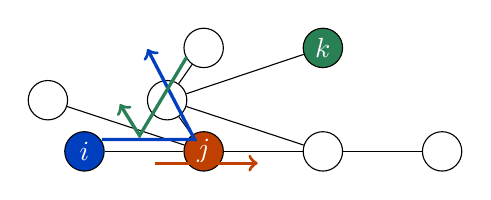
\begin{tikzpicture}
        \node[agent1](v1) at (0.0, 0.0) {$i$};
        \node[agent2,right=\edgesize of v1](v2) {$j$};
        \node[vertex,right=\edgesize of v2](v3) {};
        \node[vertex,right=\edgesize of v3](v4) {};
        \node[vertex](v5) at (1.05,0.65) {};
        \node[vertex,above=0.8cm of v2](v6) {};
        \node[agent3,above=0.8cm of v3](v7) {$k$};
        \node[vertex,left=\edgesize of v5](v8) {};
        %
        \foreach \u / \v in {v1/v2,v2/v3,v3/v4,v2/v5,v3/v5,v5/v6,v5/v7,v2/v8}
        \draw[line] (\u) -- (\v);
        % agent 1
        \draw[line,->,color={rgb:red,0;green,1;blue,3},very thick]
        (0.22, 0.15) -- (1.4, 0.15) -- (0.8, 1.3);
        % agent 2
        \draw[line,->,color={rgb:red,3;green,1;blue,0},very thick] (0.9, -0.15) -- (2.2, -0.15);
        % agent 3
        \draw[line,->,color={rgb:red,1;green,3;blue,2},very thick]
        (1.3, 1.2) -- (0.7, 0.2) -- (0.45, 0.6);
      \end{tikzpicture}
    \end{minipage}
    &
      \begin{minipage}[t]{\colwidth}
        \centering
        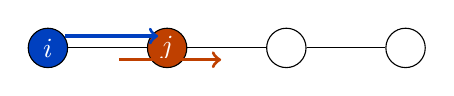
\begin{tikzpicture}
          \node[agent1](v1) at (0.0, 0.0) {$i$};
          \node[agent2,right=\edgesize of v1](v2) {$j$};
          \node[vertex,right=\edgesize of v2](v3) {};
          \node[vertex,right=\edgesize of v3](v4) {};
          %
          \foreach \u / \v in {v1/v2,v2/v3,v3/v4}
          \draw[line] (\u) -- (\v);
          %
          % agent 1
          \draw[line,->,color={rgb:red,0;green,1;blue,3},very thick] (0.22, 0.15) -- (1.4, 0.15);
          % agent 2
          \draw[line,->,color={rgb:red,3;green,1;blue,0},very thick] (0.9, -0.15) -- (2.2, -0.15);
        \end{tikzpicture}
      \end{minipage}
  \end{tabular}
  \caption{
    Examples of unreachable potential deadlocks.
    \emph{left}: cyclic; $((i, j, k), (3, 1, 2))$.
    \emph{right}: terminal; $(i, j, 2)$.
  }
  \label{fig:counterexamples}
\end{figure}


\section{Solution Analysis}
\label{sec:solution-analysis}
Given a set of paths, our first question is to determine whether it is a solution.
This section derives a necessary and sufficient condition for solutions.
For this purpose, we introduce four types of \emph{deadlocks}, categorized as; \emph{cyclic} or \emph{terminal}; \emph{potential} or \emph{reachable}.
Informally, a cyclic deadlock is a situation where agent $i$ wants to move to the current vertex of $j$, who wants to move to the current vertex of $k$, who wants to move to ... of $i$.
A terminal deadlock is a situation where agent $i$ reaches its destination and blocks the progress of another agent $j$.
A potential deadlock is called reachable when there exists an execution schedule leading to the deadlock.

\begin{definition}[potential cyclic deadlock]
  Given an OTIMAPP instance and a set of paths $\{ \path{1}, \ldots \path{N} \}$, a \emph{potential cyclic deadlock} is a pair of tuples $\left((i, j, k, \ldots, l), (t_i, t_j, t_k, \ldots, t_l)\right)$ such that $\loc{i}{t_i+1} = \loc{j}{t_j} \land \loc{j}{t_j+1} = \loc{k}{t_k} \land \ldots \land \loc{l}{t_l+1} = \loc{i}{t_i}$.
  The elements of the first tuple are without duplicates.
  \label{def:potential-cycle-deadlock}
\end{definition}

\begin{definition}[potential terminal deadlock]
  Given an OTIMAPP instance and a set of paths $\{ \path{1}, \ldots \path{N} \}$, a \emph{potential terminal deadlock} is a tuple $(i, j, t_j)$ such that $\path{i}\left[-1\right] = \path{j}[t_j]$ and $i \neq j$.
  \label{def:potential-terminal-deadlock}
\end{definition}

\begin{definition}[reachable cyclic deadlock]
  A potential cyclic deadlock $\left((i, j, \ldots, l), (t_i, t_j, \ldots, t_l)\right)$ is \emph{reachable} when there is an execution schedule leading to a situation where $\clock_i = t_i \land \clock_j = t_j \land \ldots \land \clock_l = t_l$.
  This deadlock is called a \emph{reachable cyclic deadlock}.
  \label{def:reachable-cycle-deadlock}
\end{definition}

\begin{definition}[reachable terminal deadlock]
  A potential terminal deadlock $\left(i, j, t_j\right)$ is \emph{reachable} when there is an execution schedule leading to a situation where $\clock_i = |\path{i}| \land \clock_j = t_j - 1$.
  This deadlock is called a \emph{reachable terminal deadlock}.
  \label{def:reachable-terminal-deadlock}
\end{definition}

We refer to both reachable (or potential) cyclic/terminal deadlocks by reachable (resp. potential) deadlocks and simply use ``deadlock'' whenever the context is obvious.
At least one execution schedule is required to verify whether a potential deadlock is reachable.
For instance, in Fig.~\ref{fig:example} (left), a schedule $(i, i, \ldots )$ is evidence.
A potential deadlock is not always reachable as illustrated in Fig.~\ref{fig:counterexamples}.

\begin{theorem}[necessary and sufficient condition]
  Given an OTIMAPP instance, a set of path $\{ \path{1}, \ldots, \path{N} \}$ is a solution if and only if there are (1)~no reachable terminal deadlocks and (2)~no reachable cyclic deadlocks.
  \label{thrm:necessary-sufficient}
\end{theorem}
\begin{sketch}
  Verifying that they are necessary is straightforward.
  To see that they are sufficient, consider a potential function $\phi \defeq \sum_{i \in A} (|\path{i}| - \clock_i)$ defined over a configuration $\{ \clock_1, \ldots, \clock_N \}$.
  Observe that $\phi$ is non-increasing and $\phi=0$ means that all agents have reached their goals.
  Furthermore, when $\phi > 0$, $\phi$ is guaranteed to decrease if each agent is activated at least once.
\end{sketch}

\section{Computational Complexity}
\label{sec:complexity}
This section studies the complexity of OTIMAPP.
In particular, we address two questions: the difficulty to find solutions (Sec.~\ref{sec:complexity:finding}) and the difficulty to verify solutions (Sec.~\ref{sec:complexity:verification}).
Our main results are that both problems are computationally intractable;
the former is NP-hard and the latter is co-NP-complete.
Both proofs are based on reductions from the 3-SAT problem, deciding satisfiability for a formula in conjunctive normal form with three literals in each clause.

\subsection{Finding Solutions}
\label{sec:complexity:finding}
We distinguish directed graphs and undirected graphs to analyze the complexity.
The following proof is partially inspired by the NP-hardness of MAPF on digraphs~\cite{nebel2020computational}.

\begin{theorem}[complexity on digraphs]
  OTIMAPP on \emph{directed} graphs is NP-hard.
  \label{thrm:np-hard-directed}
\end{theorem}
\begin{proof}
  The proof is a reduction from the 3-SAT problem.
  Figure~\ref{fig:3-sat-finding} is an example of the reduction from a formula $(x_1 \lor x_2 \lor \lnot x_3) \land (\lnot x_1 \lor x_2 \lor x_3)$.

  \medskip
  \noindent
  \emph{A. Construction of an OTIMAPP instance.}
  We introduce two gadgets, called \emph{variable decider} and \emph{clause constrainer}.
  The OTIMAPP instance contains one variable decider for each variable and one clause constrainer for each clause.

  The variable decider for a variable $x_i$ assigns $x_i$ to true or false.
  This gadget contains one agent $\chi_i$ with two paths to reach its goal: \emph{left} or \emph{right}.
  Taking a left path corresponds to assigning $x_i$ to false, and vice versa.
  For the $j$-th clause $C^j$ in the formula, when its $k$-th literal is either $x_i$ or $\lnot x_i$, we further add one agent $c^j_k$ to the gadget.
  Its start and goal are positioned on the \emph{right} side from $\chi_i$ when the literal is a negation; otherwise, on the \emph{left} side.
  When several such agents are positioned on one side, let them connect (see the gadget for $x_2$).
  $c^j_k$ has two alternate paths to reach its goal: a path within the variable decider or a path via a clause constrainer.
  The former is available only when $\chi_i$ takes a path of the opposite direction to avoid a reachable cyclic deadlock.

  The clause constrainer for a clause $C^j$ connects the start and the goal of $c^j_k$.
  The gadget contains a triangle.
  Each literal $c^j_k$ enters this triangle from a distinct vertex and exits from another vertex.
  As a result, this gadget prevents three literals in $C^j$ from being false simultaneously; if not so, three agents enter the gadget and there is a reachable cyclic deadlock.

  The number of agents, vertices, and edges are all polynomial with respect to the size of the formula.

  \medskip
  \noindent
  \emph{B. The formula is  satisfiable if OTIMAPP has a solution}:
  the use of one clause constrainer by three agents leads to a reachable cyclic deadlock.
  Thus, at least one literal for each clause becomes true in any OTIMAPP solution.

  \medskip
  \noindent
  \emph{C. OTIMAPP has a solution if the formula is satisfiable}:
  If satisfiable, let $\chi_i$ take a path that follows the assignment.
  Let $c^j_k$ take a path within the variable decider when $\chi_i$ takes the opposite direction; otherwise, use the clause constrainer.
  Since three agents never enter one clause constrainer due to satisfiability, those paths constitute a solution.
\end{proof}

For undirected graphs, we limit solutions to those containing only simple paths.%
\footnote{
  We recently proved that it is NP-hard for the general case of undirected graphs.
  The formal proof will appear soon.
}

{
  \begin{figure}[t]
    \centering
    \includegraphics[width=1\linewidth]{fig/raw/3-sat.pdf}
    \caption{
      An OTIMAPP instance reduced from the 3-SAT formula $(x_1 \lor x_2 \lor \lnot x_3) \land (\lnot x_1 \lor x_2 \lor x_3)$.
    }
    \label{fig:3-sat-finding}
  \end{figure}
}

{
\begin{figure}
  \centering
  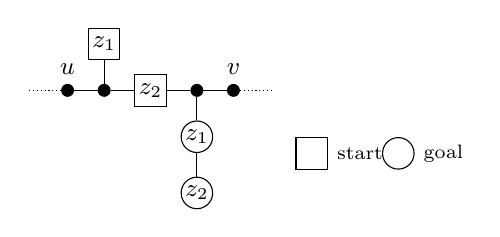
\begin{tikzpicture}
    \newcommand{\edgesize}{0.3cm}
    \newcommand{\edgesizehalf}{0.15cm}
    \newcommand{\edgesizethreetwo}{0.35cm}
    \newcommand{\longedgesize}{1.2cm}
    \small
    \tikzset{
      satnode/.style={vertex, minimum size=0.15cm, fill=black},
      start-node/.style={vertex, minimum size=0.4cm,rectangle},
      goal-node/.style={vertex, minimum size=0.4cm},
      line-c1/.style={brown,->},
      line-c2/.style={lightgray,->},
    }
    {
      \node[satnode, label=above:{\small $u$}](v1) at (0.0, 0.0) {};
      \node[satnode, right=\edgesize of v1](v2) {};
      \node[start-node, right=\edgesize of v2](v3) {$z_2$};
      \node[satnode, right=\edgesize of v3](v4) {};
      \node[satnode, right=\edgesize of v4,label=above:{\small $v$}](v5) {};
      \node[start-node, above=\edgesize of v2](v6) {$z_1$};
      \node[goal-node, below=\edgesize of v4](v7) {$z_1$};
      \node[goal-node, below=\edgesize of v7](v8) {$z_2$};
      %
      \foreach \u / \v in {v1/v2,v2/v3,v3/v4,v4/v5,v6/v2,v4/v7,v7/v8}
      \draw[line] (\u) -- (\v);
      \draw[line, densely dotted] (v1) -- ($(v1) + (-0.5, 0.0)$);
      \draw[line, densely dotted] (v5) -- ($(v5) + (0.5, 0.0)$);
      %
      \node[start-node, label=right:{\scriptsize start}](label-s) at (3.1, -0.8){};
      \node[goal-node, label=right:{\scriptsize goal}](label-g) at (4.2, -0.8){};
    }
  \end{tikzpicture}
  \caption{
    A \textit{oneway constrainer}.
    This gadget transforms an undirected edge $(u, v)$ to a directed one.
    Any agent is allowed to move only the way from $u$ to $v$ when limiting solutions to simple paths.
  }
  \label{fig:undirected-gadget}
\end{figure}
}


\begin{theorem}[complexity on undirected graphs]
  For OTIMAPP on \emph{undirected} graphs, it is NP-hard to find a solution with \emph{simple} paths.
  \label{thrm:np-hard-undirected}
\end{theorem}
\begin{sketch}
  We add a new gadget called \textit{oneway constrainer}, which transforms an undirected edge to a virtually directed one, to the proof of the NP-hardness on digraphs (Thm.~\ref{thrm:np-hard-directed}).
  We derive the claim by replacing all directed edges, except for bidirectional edges, with this gadget.
  Figure~\ref{fig:undirected-gadget} illustrates it, including two new agents: $z_1$ and $z_2$.
  In this gadget, any agents outside of the gadget are allowed to move only in the direction from $u$ to $v$.
\end{sketch}

\subsection{Verification}
\label{sec:complexity:verification}
The co-NP completeness of the verification relies on the following lemma, stating that finding cyclic deadlocks is computationally intractable.
Its entire proof is delivered in the Appendix.
\begin{lemma}[complexity of detecting cyclic deadlocks]
  Determining whether a set of paths contains either reachable or potential cyclic deadlocks is NP-complete.
  \label{lemma:deadlock-np-comp}
\end{lemma}
We then derive the complexity result since a solution has no reachable deadlocks.
\begin{theorem}[complexity of verification]
  Verifying a solutions of OTIMAPP is co-NP-complete.
  \label{thrm:co-np-hard:verification}
\end{theorem}
\begin{proof}
  Thm.~\ref{thrm:necessary-sufficient} states that a solution has no reachable terminal/cyclic deadlocks.
  Verifying no terminal deadlocks is in co-NP; a terminal deadlock is verified in polynomial time with an execution schedule.
  Verifying no potential deadlocks is co-NP-complete according to Lemma~\ref{lemma:deadlock-np-comp}.
\end{proof}


\section{Solvers}
\label{sec:solvers}
We now focus on how to solve OTIMAPP.
In practice, it is difficult to use the necessary and sufficient condition (Thm.~\ref{thrm:necessary-sufficient}) because we have to find corresponding schedules.
This motivates to build a relaxed sufficient condition.
\begin{theorem}[relaxed condition]
  Given an OTIMAPP instance, a set of path $\{ \path{1}, \ldots, \path{N} \}$ is a solution when there are
  (1)~no use of other goals, i.e., $g_j \not\in \path{i}$ for all $i \neq j$ except for $s_i = g_j$, and
  (2)~no potential cyclic deadlocks.
  \label{thrm:sufficient}
\end{theorem}
It is straightforward to see that the above conditions are respectively sufficient for the two conditions in Thm.~\ref{thrm:necessary-sufficient}.
Given a set of paths, ``no use of other goals'' is easy to check while ``no potential cyclic deadlocks'' is intractable to compute (Lemma~\ref{lemma:deadlock-np-comp}).
Nevertheless, \emph{detecting potential cyclic deadlock is the heart of solving OTIMAPP}.
Thus, we first explain how to detect potential cyclic deadlocks.
After that, two algorithms to solve OTIMAPP are presented.

\subsection{Detection of Potential Deadlocks}
Due to the space limit, we only describe the intuition behind the algorithm.
The details are in the Appendix (Alg.~\ref{algo:detecting-deadlock}).
We first introduce a \emph{fragment}, a candidate of potential cyclic deadlocks.
\begin{definition}[fragment]
  Given a set of paths $\{\path{1},$$\ldots,$$\path{N}\}$, a \emph{fragment} is a tuple $\left((i, j, k, \ldots, l), (t_i, t_j, t_k, \ldots, t_l)\right)$ such that $\loc{i}{t_i+1}=\loc{j}{t_j} \land \loc{j}{t_j+1} = \loc{k}{t_k} \land \ldots = \loc{l}{t_l}$.
  The elements of the first tuple are without duplicates.
  \label{def:fragment}
\end{definition}
\noindent
We say that a fragment \emph{starts} from a vertex $u$ when $\loc{i}{t_i} = u$ and a fragment \emph{ends} at a vertex $v$ when $\loc{l}{t_l+1} = v$.
A fragment that ends at its start (i.e., $\loc{l}{t_l+1} = \loc{i}{t_i}$) is a potential cyclic deadlock.

{
  \newcommand{\f}[3]{\m{\left[(#1), (#2), (#3)\right]}}
  \begin{table}[t]
    \centering
    {
    \footnotesize
    \begin{tabular}{rrl}
      \toprule
      induction & key & new fragments
      \\ \midrule
      $\{\pi_1\}$
          & $u$ & \f{1}{1}{u,v} \\
          & $v$ & \f{1}{2}{v,w}
          %
      \\ \midrule
      %
      $\{\pi_1, \pi_2\}$
          & $u$ & \f{1,2}{1,1}{u,v,x} \\
          & $v$ & \f{2}{1}{v,x} \\
          & $x$ & \f{2}{2}{x,y}
          %
      \\ \midrule
      $\{\pi_{1}, \pi_{2}, \pi_{3}\}$
          & $u$ & \textcolor{blue}{\f{1,2,3}{1,1,2}{u,v,x,u}} \\
          & $v$ & \f{2,3}{1,2}{v,x,u} \\
          & $x$ & \f{3}{2}{x,u}, \f{3,1}{2,1}{x,u,v}\\
          & $z$ & \f{3}{1}{z,x}, \f{3,2}{1,2}{z,x,y}
      \\ \bottomrule
    \end{tabular}
    }
    \caption{
      Example of detecting potential cyclic deadlocks.
      We describe the update of \tablefrom for $\path{1} = (u, v, w), \path{2} = (v, x, y), \path{3} = (z, x, u)$.
      The table uses $[(\text{agents}), (\text{progress indexes}), (\text{path})]$ as a notation of fragment,  where ``path'' is a corresponding sequence of vertices of the fragment.
      The algorithm halts with a blue-colored fragment, a detected potential cyclic deadlock.
    }
    \label{table:update-tablefrom}
  \end{table}
}


Using fragments, we construct an algorithm to detect a potential cyclic deadlock in a set of paths if it exists.
This is based on induction on \path{i}.
The induction hypothesis for $i$ is that there are no potential cyclic deadlocks for $\{ \path{1}, \ldots, \path{i-1} \}$ and all fragments for them are identified.
All new fragments about \path{i} are categorized into three groups:
(1)~a fragment only with \path{i},
(2)~a fragment that extends existing fragments, and
(3)~a fragment that connects existing two fragments.
In either case, if a newly created fragment ends at its start, this is a deadlock.

The algorithm realizes this procedure by managing two tables that store fragments: \tablefrom and \tableto.
Both tables take one vertex as a key.
One entry in \tablefrom stores all fragments starting from the vertex.
One entry in \tableto stores all fragments ending at the vertex.
Table~\ref{table:update-tablefrom} presents an example to detect deadlocks.

\subsection{Prioritized Planning (PP)}
Prioritized planning~\cite{erdmann1987multiple,silver2005cooperative} is neither complete nor optimal, but it is computationally cheap hence a popular approach to MAPF.
It plans paths sequentially while avoiding collisions with previously planned paths.
Instead of inter-agent collisions, solvers for OTIMAPP have to care about potential cyclic deadlocks.

Algorithm~\ref{algo:pp} is prioritized planning for OTIMAPP, named \emph{PP}.
When planning a single-agent path, PP avoids using (1)~goals of other agents and (2)~edges causing potential cyclic deadlocks~[Line~\ref{algo:pp:planning}].
The latter is detected by storing all fragments created by previously computed paths.
For this purpose, PP uses the adaptive version of Alg.~\ref{algo:detecting-deadlock} [Line~\ref{algo:pp:register}] in the Appendix.
A path satisfying the constraints can be found by ordinary pathfinding algorithms.
If not, PP returns \FAILURE.
The correctness of PP is derived from Thm.~\ref{thrm:sufficient}.

{
  \begin{algorithm}[tb!]
  \caption{PP: Prioritized Planning}
  \label{algo:pp}
  \textbf{Input}:~an OTIMAPP instance\\
  \textbf{Output}:~a solution $\{ \path{1}, \ldots, \path{N} \}$ or \FAILURE
  \begin{algorithmic}[1]
    \State $\tablefrom, \tableto \leftarrow \emptyset$
    \For{$i = 1\ldots~|A|$}
    \State $\path{i} \leftarrow
    \begin{aligned}[t]
      &\text{a path for agent}~i~\text{while avoiding the use of}
      \\
      &\cdot~g_j, \forall j \neq i, \text{except for}~s_i
      \\
      &\cdot~(u, v) \in E~\text{s.t.}~\exists \theta \in \tableto[u]~\text{and}~\theta~\text{starts from}~v
      \\
      &\hspace{0.3cm}\triangleright\text{avoiding cyclic deadlocks for}~\path{j}, j < i
    \end{aligned}$
    \label{algo:pp:planning}
    \IFSINGLE{\path{i} is not found}{\Return \FAILURE}
    \State update \tablefrom and \tableto with \path{i} using Algorithm~\ref{algo:detecting-deadlock}
    \label{algo:pp:register}
    \EndFor
    \State \Return $\{ \path{1}, \ldots, \path{N} \}$
  \end{algorithmic}
\end{algorithm}
}

PP is simple but incomplete.
In particular, the planning order of agents is crucial; an instance may be solved or may not be solved as illustrated in Fig.~\ref{fig:prioritization}.
One resolution is repeating PP with random priorities until the problem is solved; let call this PP$^+$.
However, finding good orders can be challenging because there are $|A|!$ patterns.
This motivates us to develop a search-based solver, described in the next.

\begin{figure}[tb!]
  \centering
  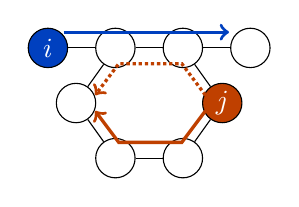
\begin{tikzpicture}
    \newcommand{\edgesize}{0.6cm}
    % \scriptsize
    %
    \node[agent1](v1) at (0.0, 0.0) {$i$};
    \node[vertex, right=\edgesize of v1.center](v2) {};
    \node[vertex, right=\edgesize of v2.center](v3) {};
    \node[vertex, right=\edgesize of v3.center](v4) {};
    \node[vertex](v5) at ($(v2) + (-0.5,  -0.7)$) {};
    \node[agent2](v6) at ($(v3) + ( 0.5,  -0.7)$) {$j$};
    \node[vertex](v7) at ($(v2) + ( 0.0,  -1.4)$) {};
    \node[vertex](v8) at ($(v3) + ( 0.0,  -1.4)$) {};
    %
    \foreach \u / \v in {v1/v2,v2/v3,v3/v4,v2/v5,v3/v6,v5/v7,v6/v8,v7/v8}
    \draw[line] (\u) -- (\v);
    %
    \draw[line,->,color={rgb:red,0;green,1;blue,3},very thick]
    (0.2, 0.2) -- (2.3, 0.2);
    \draw[line,->,color={rgb:red,3;green,1;blue,0},very thick, densely dotted]
    (2.0, -0.6) -- (1.7, -0.2) -- (0.9, -0.2) -- (0.6, -0.6);
    \draw[line,->,color={rgb:red,3;green,1;blue,0},very thick]
    (2.0, -0.8) -- (1.7, -1.2) -- (0.9, -1.2) -- (0.6, -0.8);
  \end{tikzpicture}
  \caption{
    Example that the planning order affects the solvability.
    When $i$ plans prior to $j$, PP results in success with solid lines.
    PP fails if $j$ plans first and takes the dotted line.
  }
  \label{fig:prioritization}
\end{figure}


\subsection{Deadlock-based Search (DBS)}
We present \emph{deadlock-based search (DBS)} to solve OTIMAPP, based on a popular search-based MAPF solver called \emph{conflict-based search (CBS)}~\cite{sharon2015conflict}.
CBS uses a two-level search.
The high-level search manages collisions between agents.
When a collision occurs between two agents at some time and location, two possible resolutions are depending on which agent gets to use the location at that time.
Following this observation, CBS constructs a binary tree where each node includes constraints prohibiting to use space-time pairs for certain agents.
In the low-level search, agents find a single path constrained by the corresponding high-level node.

Instead of collisions, DBS considers potential cyclic deadlocks.
When detecting a deadlock in a set of paths, a resolution is that one of the agents in the deadlock avoids using the edge.
Thus, the constraints identify which agents prohibit using which edges in which orientation.

{
  \begin{algorithm}[tb!]
  \caption{DBS: Deadlock-based Search}
  \newcommand{\OPEN}{\m{\mathit{OPEN}}}
  \label{algo:cp}
  \textbf{Input}:~an OTIMAPP instance\\
  \textbf{Output}:~a solution $\{ \path{1}, \ldots, \path{N} \}$ or \FAILURE
  \begin{algorithmic}[1]
    \State $R.\mathit{constraints} \leftarrow \emptyset$
    \label{algo:cp:root:constraints}
    \State $R.\mathit{paths} \leftarrow$~find paths with ``no use of other goals''
    \label{algo:cp:root:paths}
    \State insert $R$ to \OPEN
    \label{algo:cp:root:insert}
    \Comment \OPEN: priority queue
    \While{$\OPEN \neq \emptyset$}
    \label{algo:cp:while}
    \State $N \leftarrow \OPEN.\mathit{pop}()$
    \label{algo:cp:pop}
    \State $C \leftarrow$ get constraints of $N$ using Algorithm~\ref{algo:detecting-deadlock}
    \label{algo:cp:get-constraints}
    \IFSINGLE{$C = \emptyset$}{\Return $N.\mathit{paths}$}
    \label{algo:cp:return-solution}
    \For{$(i, u, v) \in C$}
    \label{algo:cp:exapnd:for}
    \State $\p{N} \leftarrow
    \begin{aligned}[t] \{
      &\mathit{constraints}: N.\mathit{constraints} + (i, u, v),\\
      &\mathit{paths}: N.\mathit{paths}\}
    \end{aligned}$
    \State update \path{i} in $\p{N}.\mathit{paths}$ to follow $\p{N}.\mathit{constraints}$
    \label{algo:cp:update}
    \IFSINGLE{\path{i} is found}{insert $\p{N}$ to \OPEN}
    \EndFor
    \label{algo:cp:exapnd:for:end}
    \EndWhile
    \label{algo:cp:while:end}
    \State \Return \FAILURE
    \label{algo:cp:return-failure}
  \end{algorithmic}
\end{algorithm}
}

Algorithm~\ref{algo:cp} describes the high-level search of DBS.
Each node in the high-level search contains \emph{constraints}, a list of tuples consisting of one agent and two vertices (representing ``from vertex'' and ``to vertex''), and \emph{paths} as a solution candidate.
The root node does not have any constraints~[Line~\ref{algo:cp:root:constraints}].
Its paths are computed following ``no use of other goals'' of Thm.~\ref{thrm:sufficient}~[Line~\ref{algo:cp:root:paths}].
Then, the node is inserted into a priority queue \open~[Line~\ref{algo:cp:root:insert}].
In the main loop [Line~\ref{algo:cp:while}--\ref{algo:cp:while:end}], DBS repeats;
(1)~Picking up one node~[Line~\ref{algo:cp:pop}].
(2)~Checking a deadlock and creating constraints~[Line~\ref{algo:cp:get-constraints}].
(3)~Returning a solution if the paths contain no deadlocks~[Line~\ref{algo:cp:return-solution}].
(4)~If not, creating successors and inserting them to \open~[Line~\ref{algo:cp:exapnd:for}--\ref{algo:cp:exapnd:for:end}].
DBS returns \FAILURE when \open becomes empty~[Line~\ref{algo:cp:return-failure}].
We complement several details below.

{
\smallskip
\newcommand{\myitemize}[2]{\noindent{$\blacktriangleright$~\emph{#1}:}#2\smallskip}

\myitemize{Line~\ref{algo:cp:pop}}{
  \open is a priority queue and needs the order of nodes.
  DBS works in any order but good orders reduce the search effort.
  As effective heuristics, we use the descending order of the number of deadlocks with two agents, which is computed within a reasonable time.}

\myitemize{Line~\ref{algo:cp:get-constraints}}{
  Let $((i, j, k, \ldots, l),$$(t_i, t_j, t_k, \ldots, t_l))$ be a returned deadlock by Alg.~\ref{algo:detecting-deadlock}.
  Then, create constraints $(i, \loc{i}{t_i}, \loc{i}{t_i+1}), (j, \loc{j}{t_j}, \loc{j}{t_j+1}), \ldots, (l, \loc{l}{t_l}, \loc{l}{t_l+1})$.}

\myitemize{Line~\ref{algo:cp:update}}{
  forces one path \path{i} in the node to follow the new constraints.
  This low-level search must follow ``no use of other goals,'' furthermore, all edges in the constraints for $i$.
  If not found, DBS discards the corresponding successor.}
}

\begin{theorem}[DBS]
  DBS returns a solution when solutions satisfying Thm.~\ref{thrm:sufficient} exist; otherwise returns \FAILURE.
  \label{thrm:dbs}
\end{theorem}

\paragraph{Example}
We describe an example of DBS using Fig.~\ref{fig:prioritization}.
Assume that the initial path of $i$ is the solid blue line and the path for $j$ is the dashed red line [Line~\ref{algo:cp:root:paths}].
This node is inserted into \open~[Line~\ref{algo:cp:root:insert}] and is expanded immediately~[Line~\ref{algo:cp:pop}].
There is one potential cyclic deadlock in the paths then two constraints are created: either $i$ or $j$ avoids using the shared edge~[Line~\ref{algo:cp:update}].
Two child nodes are generated, however, the node that changes $i$'s path is invalid because there is no such path without the use of the goal of $j$.
Another one is valid; $j$ takes the solid red line.
Therefore, one node is added to \open from the root node.
In the next iteration, this newly added node is expanded.
There are no potential cyclic deadlocks in this node;
DBS returns its paths as a solution.

\paragraph{Optimization}
Although this paper focuses on a feasibility problem, DBS can adapt to optimization problems.
As objective functions, total path length and maximum path length in a solution can be defined.
Those optimization problems are solved optimally by DBS when it prioritizes high-level search nodes with smaller scores, as commonly done in CBS.
Note that metrics that assess time aspects such as total traveling time used in MAPF studies are significantly affected by execution schedules; the adaptation is not trivial.

\section{Evaluation}
\label{sec:eval}
This section empirically demonstrates that OTIMAPP solutions are computable to some extent (Sec.~\ref{sec:stress-test}) and they are useful in adverse environments about timings (Sec.~\ref{sec:delay-tolerance}) through the simulation experiments.
We also present OTIMAPP execution with robots (Sec.~\ref{sec:demo}).
The simulator was coded in C++ and the experiments were run on a desktop PC with Intel Core~i9 \SI{2.8}{\giga\hertz} CPU and \SI{64}{\giga\byte} RAM.

\subsection{Stress Test}
\label{sec:stress-test}
\paragraph{Setup}
Each solver was tested with a timeout of \SI{5}{\minute} on four-connected undirected grids picked up from~\cite{stern2019def}, as a graph $G$.
We also tested random graphs, shown in the Appendix.
All instances were generated by setting a start $s_i$ and a goal $g_i$ randomly while ensuring that $s_i$ and $g_i$ have at least one path without the use of other goals; otherwise, it violates ``no use of other goals'' of Thm.~\ref{thrm:sufficient}.
Note that unsolvable instances might still be included.

{
  \setlength{\tabcolsep}{0pt}
  \newcommand{\colwidth}{0.32\hsize}
  %
  \newcommand{\plotStress}[1]{
    \begin{minipage}[t]{\colwidth}
      \centering
      \IfFileExists{fig/raw/stress-#1.pdf}{\includegraphics[width=1.0\linewidth]{fig/raw/stress-#1.pdf}}{}
    \end{minipage}
  }
  %
  \newcommand{\plotCactus}[1]{
    \begin{minipage}[t]{\colwidth}
      \centering
      \IfFileExists{fig/raw/cactus-#1.pdf}{\includegraphics[width=1.0\linewidth]{fig/raw/cactus-#1.pdf}}{}
    \end{minipage}
  }
  \newcommand{\plotProfiling}[1]{
    \begin{minipage}[t]{\colwidth}
      \centering
      \IfFileExists{fig/raw/profiling-#1.pdf}
      {\includegraphics[width=0.95\linewidth,right]{fig/raw/profiling-#1.pdf}}{}
    \end{minipage}
  }
  %
  \newcommand{\headerGrid}[4]{
    \begin{minipage}[t]{\colwidth}
      \centering
      {
        \setlength{\tabcolsep}{1pt}
        \renewcommand{\arraystretch}{0.8}
        \begin{tabular}{lr}
          {\scriptsize\field{#1}}
          & \multirow{2}{*}{\includegraphics[width=0.23\linewidth]{fig/raw/#1.pdf}}\\
          {\tiny\m{#2\stimes #3~(#4)}} &
        \end{tabular}
      }
    \end{minipage}
  }
  %
  \begin{figure}[tb!]
    \centering
    \begin{tabular}[t]{ccc}
      \headerGrid{random-32-32-10}{32}{32}{922}
      & \headerGrid{random-64-64-10}{64}{64}{3687}
      & \headerGrid{den520d}{256}{257}{28178}
        \medskip\\
      \plotStress{random-32-32-10}
      & \plotStress{random-64-64-10}
      & \plotStress{den520d}
      \\
      \plotCactus{random-32-32-10}
      & \plotCactus{random-64-64-10}
      & \plotCactus{den520d}
      \\
      \plotProfiling{random-32-32-10}
      & \plotProfiling{random-64-64-10}
      & \plotProfiling{den520d}
    \end{tabular}
    \caption{
      Stress test on 4-connected grids.
      The success rate is based on 25 identical instances.
      DBS$^\ast$ includes detected instances that are unsolvable for DBS before timeout, which is not possible for PP$^{(+)}$.
      We also present accumulated runtime with a fixed number of agents over 100 instances, and runtime profiling (median) of each solver over success instances for both solvers.
    }
    \label{fig:stress-test}
  \end{figure}
}


\paragraph{Result}
Fig.~\ref{fig:stress-test} presents the results.
The main findings are:
(1)~Both solvers can solve instances with tens of agents in various maps within a reasonable time.
(2)~PP often fails due to priority orders (e.g., Fig.~\ref{fig:prioritization}) while PP$^+$ and DBS can overcome such limitations to some extent.
(3)~A bottleneck of each solver is the procedure of detecting potential cyclic deadlocks, an NP-hard problem (Lemma.~\ref{lemma:deadlock-np-comp}).
This also leads to similar success rates of PP$^+$ and DBS.

\subsection{Delay Tolerance}
\label{sec:delay-tolerance}
We next show that OTIMAPP solutions (if found) are useful in a simulated environment with stochastic delays of agents' moves built on conventional MAPF, called MAPF-DP (with Delay Probabilities)~\cite{ma2017multi}.
Given a graph and start-goal pairs for each agent, the aim of MAPF is to move agents to their goals without collisions.
Collisions occur when two agents occupy the same vertex or traverse the same edge simultaneously.
Time is discrete.
All agents synchronously take actions, i.e., either move to an adjacent vertex or stay at the current location.
MAPF-DP emulates the imperfect execution of MAPF by introducing the possibility $p_i$ of unsuccessful moves for agent $i$ (remaining there).

\paragraph{Setup}
The delay probabilities $p_i$ were chosen uniformly at random from $[0, \bar{p}]$, where $\bar{p}$ is the upper bound of $p_i$.
The higher $\bar{p}$ means that agents delay often, and vice versa.
The metric is the total traveling time of agents; smaller values mean less wasting time at runtime.
We tested the following two as baselines:
(1)~MCPs~\cite{ma2017multi} force agents to preserve order relations of visiting one vertex in an offline MAPF plan at runtime.
The plan was obtained by ECBS~\cite{barer2014suboptimal}.
(2)~Causal-PIBT~\cite{okumura2021time} is online time-independent planning, that is, each agent repeats one-step planning and action adaptively to surrounding current situations.
The other details are in the Appendix.

\paragraph{Result}
Table~\ref{table:result-delay} shows that the execution of OTIMAPP solutions outperforms the alternatives.
This is because:
(1)~Unlike MCPs, OTIMAPP solutions are free from temporal dependencies of offline plans that one agent delays are possibly fatal.
(2)~Unlike Causal-PIBT, agents follow long-term plans and avoid possible congested locations.

\paragraph{Discussion}
Although finding OTIMAPP solutions is challenging, Table~\ref{table:result-delay} motivates us to compute them.
Meanwhile, the other approaches can solve larger instances with more agents (e.g., $|A|=200$) and with much smaller planning time than solving OTIMAPP.
Moreover, there are situations where OTIMAPP has no solutions while the others can find feasible plans because OTIMAPP assumes no intervention at runtime.
One future direction pursues to fill these gaps.

{
  \setlength{\tabcolsep}{1.2mm}
  \newcommand{\ci}[1]{\tiny(#1)}
  \newcommand{\w}[1]{\textbf{#1}}
  \begin{table}[t]
    \centering
    {
    \small
    \begin{tabular}{lrlrlrl}
      \toprule
      $|A|=35$
      & \multicolumn{2}{c}{$\bar{p}=0.2$}
      & \multicolumn{2}{c}{$\bar{p}=0.5$}
      & \multicolumn{2}{c}{$\bar{p}=0.8$}
        %
      \\\midrule
      MCPs+ECBS & 1015 & \ci{1004,1026} & 1422 & \ci{1404,1440} & 2551 & \ci{2507,2596}\\
      Causal-PIBT & 986 & \ci{976,995} & 1238 & \ci{1225,1250} & 1841 & \ci{1816,1866} \\
      OTIMAPP & \w{941} & \ci{931,951} & \w{1178} & \ci{1165,1190} & \w{1730} & \ci{1707,1752}
      \\\toprule
      $\bar{p}=0.5$
      & \multicolumn{2}{c}{$|A|=20$}
      & \multicolumn{2}{c}{$|A|=40$}
      & \multicolumn{2}{c}{$|A|=60$}
      %
      \\\midrule
      MCPs+ECBS & 724 & \ci{711,736} & 1698 & \ci{1678,1716} & 2938 & \ci{2911,2964} \\
      Causal-PIBT & 662 & \ci{653,671} & 1466 & \ci{1453,1479} & 2425 & \ci{2405,2444} \\
      OTIMAPP & \w{639} & \ci{631,648} & \w{1395} & \ci{1383,1408} & \w{2328} & \ci{2311,2345}
      \\ \bottomrule
    \end{tabular}
    }
    \caption{
      Total traveling time on MAPF-DP.
      All settings used \field{random-32-32-10}.
      For each setting, we first picked up 10 instances that OTIMAPP solutions were found by PP$^+$.
      For each instance and approach, we then performed 50 trials while changing the random seed.
      Thus, the scores are means on 500 executions, accompanied with 95\% confidence intervals.
      \emph{upper}:~Results of changing $\bar{p}$ while fixing $|A|$.
      \emph{lower}:~Results of changing $|A|$ while fixing $\bar{p}$.
      Note that the probability that someone delays increases with more agents.
    }
    \label{table:result-delay}
  \end{table}
}

{
  \newcommand{\colwidth}{0.49\linewidth}
  \setlength{\tabcolsep}{1pt}
  \begin{figure}[t]
    \centering
    \begin{tabular}{cc}
      \begin{minipage}{\colwidth}
        \centering
        \includegraphics[width=1\hsize]{fig/raw/toio.jpg}
      \end{minipage}
      &
      \begin{minipage}{\colwidth}
        \centering
        \includegraphics[width=1\hsize]{fig/raw/afada.jpg}
      \end{minipage}
    \end{tabular}
    \caption{
      An OTIMAPP execution with $10$~robots in an $8\times 8$ grid.
      Colored arrows represent an OTIMAPP solution.
    }
    \label{fig:demo}
  \end{figure}
}


\subsection{Robot Demonstrations}
\label{sec:demo}
We present two OTIMAPP execution styles:
(1)~a \emph{centralized} control using the \emph{toio} robots (\url{https://toio.io}) and
(2)~a \emph{decentralized} one with only local interactions using a multi-robot platform~\cite{kameyama2021active}.
A solution was obtained by DBS.
Figure~\ref{fig:demo} is snapshots.
A video is available online.
In both cases, robots move without any synchronization procedures but are ensured to eventually reach their goals thanks to the nature of OTIMAPP.
Moreover, for the latter, any actor has no methods to know the entire configuration, which cannot be addressed by conventional execution strategies.

\section{Related Work}
% System deadlock
A \emph{deadlock}~\cite{coffman1971system} is a widely recognized phenomenon not limited to robotics;
a system state that several components claim resources that others hold, then block each other permanently.
Strategies to cope with deadlocks are categorized into prevention, detection/recovery, and avoidance~\cite{silberschatz2006operating,fanti2004deadlock};
\emph{OTIMAPP is prevention}.
A non-deadlock state that is ``inevitable'' to reach deadlocks is called \emph{unsafe}~\cite{silberschatz2006operating}.
Meanwhile, reachable deadlocks of OTIMAPP correspond to states that are ``possible'' to reach deadlocks.
The notion of potential terminal deadlock is related to well-formed instances of MAPF~\cite{vcap2015prioritized}, that is, for each start-goal pair, a path exists that traverses no other starts and goals.
The notion of reachable cyclic deadlock is mentioned as nonlive states/sets for deadlock management in automated manufacturing systems~\cite{fanti2004deadlock} or in a multi-robot scheduling problem~\cite{mannucci2021provably}.

% multi-agent path finding
The \emph{multi-agent pathfinding (MAPF)} problem~\cite{stern2019def} aims at finding a set of collision-free paths on a graph.
Many studies on MAPF consider timing uncertainties because they are inevitable in multi-agent scenarios.
However, current methods largely rely on additional assumptions on the travel speed of agents or assume delays to follow some probability distributions~\cite{wagner2017path,mansouri2019multi,peltzer2020stt,atzmon2020probabilistic}.
Failing to represent the inherent uncertainty in the domain means the system behavior can be unpredictable.
Alternative approaches are online intervention during execution, e.g., forcing agents to preserve temporal dependencies of offline planning via communication~\cite{ma2017multi,honig2019persistent,atzmon2020robust}.
Another direction is online time-independent planning~\cite{okumura2021time} that incrementally moves agents based on current situations.
OTIMAPP shares the concept of time independence but aims at offline planning without or less runtime effort.

In graph theory, the (vertex) disjoint path problem and its variants~\cite{robertson1985disjoint} are partly related to ours in the sense that a set of disjoint paths clearly satisfies the solution condition of OTIMAPP, but the reverse does not.

\section{Conclusion}
This paper studied a novel path planning problem called OTIMAPP, motivated by the nature of distributed environments (i.e., timing uncertainties) that multi-agent systems must address.
We focused on robotic applications in evaluation but believe that OTIMAPP can be leveraged to other resource allocation problems with mutual exclusion, e.g, distributed databases, which is our future direction.
\section*{Acknowledgments}
We thank the anonymous reviewers for their many insightful comments and suggestions.
This work was partly supported by JSPS KAKENHI Grant Numbers~20J23011, 21K11748, and 21H03423.
Keisuke Okumura thanks the support of the Yoshida Scholarship Foundation.


\bibliographystyle{named}
\bibliography{ref}

%% The Appendices part is started with the command \appendix;
%% appendix sections are then done as normal sections
\appendix
% \onecolumn
\subsection{Prompt Template}
\label{app1}

Figs. \ref{appendix:prompt1}-\ref{appendix:prompt3} (due to the page length, we break it into three parts) show the prompt design for the information extraction in the context of construction project scheduling. 

\begin{figure}[t]
    \vspace{-4.5cm}
    \centering
    \begin{tcolorbox}[colback=gray!10!white, colframe=gray!50!gray, halign=left, boxrule=0.5pt, left=1mm, right=1mm, top=1mm, bottom=1mm]
    \fontsize{8pt}{8pt}\selectfont
    SYSTEM PROMPT: You are a project management assistant specializing in construction scheduling analysis. Your task is to analyze text descriptions of project changes and extract structured information about task relation changes in a construction project.
    \vspace{8pt}
    
    CONTEXT\\
    The project involves the following tasks and their relationships: \\
    \vspace{3pt}
    Task ID \textbar{} Predecessor \textbar{} Duration \textbar{} Description \textbar{} Robot Type
    \begin{itemize}
    \item T1 \textbar{} - \textbar{} 0.25 \textbar{} Move Electrical Conduit \textbar{} R1
    \item T2 \textbar{} - \textbar{} 0.25 \textbar{} Move Window Frame \textbar{} R1
    \item T3 \textbar{} - \textbar{} 0.25 \textbar{} Move Window \textbar{} R1
    \item T4 \textbar{} - \textbar{} 0.25 \textbar{} Move Duct Structural Materials \textbar{} R1
    \item T5 \textbar{} - \textbar{} 0.25 \textbar{} Move Duct \textbar{} R1
    \item T6 \textbar{} - \textbar{} 0.5 \textbar{} Drill Wall \textbar{} R4 or R2
    \item T7 \textbar{} T1, T6 \textbar{} 1 \textbar{} Install Electrical Conduit \textbar{} R5 or R2
    \item T8 \textbar{} T2 \textbar{} 1 \textbar{} Install Window Frame \textbar{} R4 or R2
    \item T9 \textbar{} T3, T8 \textbar{} 0.5 \textbar{} Install Window \textbar{} R3
    \item T10 \textbar{} T4 \textbar{} 2 \textbar{} Duct Structural Framing \textbar{} R4 or R2
    \item T11 \textbar{} T5, T10 \textbar{} 2 \textbar{} Install HVAC Duct \textbar{} R4 or R2
    \item T12 \textbar{} T7 \textbar{} 2 \textbar{} Install Wiring \textbar{} R5 or R2
    \item T13 \textbar{} T12 \textbar{} 1 \textbar{} Wall Painting \textbar{} R6
    \item T14 \textbar{} - \textbar{} 0.5 \textbar{} Construction Site Inspection \textbar{} R7
    \end{itemize}
    \vspace{8pt}
    
    The robot capabilities are listed below: \\
    \vspace{3pt}
    Robot ID \textbar{} Capabilities
    \begin{itemize}
    \item R1: Cargo container
    \item R2: High-payload, Precise parallel gripper, Normal parallel gripper
    \item R3: High-payload, Suction-based gripper
    \item R4: High-payload, Normal parallel gripper
    \item R5: Precise parallel gripper
    \item R6: Sprayer
    \item R7: Camera, IAQ sensors
    \end{itemize}
    \vspace{8pt}
    
    CONSTRAINT TYPES:
    \begin{enumerate}
    \item Task Dependency Adjustments
      \begin{itemize}
        \item Format: [task\_id, successor, +/-]
        \item task\_id: the target task
        \item successor: the successors of the target task
        \item +/-: ``+'' indicates a newly added successor, ``-'' means the dependency has been removed
      \end{itemize}
    \item Task Duration Variations
      \begin{itemize}
        \item Format: [task\_id, new\_duration]
        \item task\_id: the target task
        \item new\_duration: the new duration of the target task in hours
      \end{itemize}
    \item Task Starting Time Changes
      \begin{itemize}
        \item Format: [task\_id, start\_time\_change]
        \item task\_id: the target task
        \item start\_time\_change: the changes in start time of the target task (e.g., +2 means delayed by 2 hours; -2 means ahead by 2 hours)
      \end{itemize}
    \item Number of Robot Variations
      \begin{itemize}
        \item Format: [robot\_type\_id, robot\_number\_change]
        \item robot\_type\_id: the type of robot (e.g., R1, R2, R3, etc.)
        \item robot\_number\_change: the number changes of the robot (e.g., +1 means one more robot; -1 means one less robot)
      \end{itemize}
    \item Task Conflict Constraints
      \begin{itemize}
          \item Format: [task\_id1, task\_id2]
          \item task\_id1: the first task in the conflict
          \item task\_id2: the second task in the conflict
      \end{itemize}
    \end{enumerate}
    \end{tcolorbox}
    \caption{Prompt design for construction project scheduling - Part 1.}
    \label{appendix:prompt1}
\end{figure}


\begin{figure}[t]
    \centering
    \begin{tcolorbox}[colback=gray!10!white, colframe=gray!50!gray, halign=left, boxrule=0.5pt, left=1mm, right=1mm, top=1mm, bottom=1mm]
    \fontsize{8pt}{8pt}\selectfont
    STEP-BY-STEP INSTRUCTIONS:
    \begin{enumerate}
    \item Read through the entire description to understand the context.
    \item For each change mentioned in the description:
       \begin{itemize}
       \item[a.] Identify which task (T1-T14) or robot type (R1-R7) is being affected based on CONTEXT. 
        \begin{itemize}
          \item Be careful to distinguish between similar tasks, for example:
          \begin{itemize}
          \item T2 (Move Window Frame) vs. T3 (Move Window) vs. T8 (Install Window Frame) vs. T9 (Install Window) - These are different tasks.
          \item If text mentions ``window installation'', specifically, it refers to T9 (Install Window), not T3 or T8
          \item If text mentions "window frame installation," it refers to T8 (Install Window Frame), not T2
          \end{itemize}
        \item Be careful to distinguish between similar robots, for example:
          \begin{itemize}
          \item R2, R3, R4, and R5 are different robots. 
          \item Only R2 combines both high-payload and precise parallel gripper capabilities.
          \item If text only mentions ``high-payload and normal parallel gripper'', it refers to R4 not R2.
          \end{itemize}
       \end{itemize}
       \item[b.] Determine which constraint type (1-5) applies to the change based on CONSTRAINT TYPES.
       \item[c.] Extract the specific parameters needed for that constraint type.
       \item[d.] Format the parameters according to the required format for that constraint type.
       \end{itemize}
    \item Compile all identified changes into the JSON output format:
       \begin{itemize}
       \item[a.] Create a JSON object with a ``changes'' array.
       \item[b.] For each change, add an object with ``constraint\_type'' and ``parameters'' fields.
       \item[c.] Ensure numerical values (like durations and time changes) are formatted as numbers, not strings.
       \item[d.] Ensure task IDs, successors, and robot types are formatted as strings.
       \item[e.] For time-related values:
          \begin{itemize}
          \item Simplify all numerical values to their simplest form (e.g., 1.5 not 1.50, 2 not 2.0)
          \item Convert minutes to hours (e.g., 30 minutes = 0.5 hours, 45 minutes = 0.75 hours)
          \item Please be aware that if you identify the constraint as 3, the time change should be associated with ``+'' or ``-''. 
          \end{itemize}
       \item[g.] Please be aware that if you identify the constraint as 4, the robot change should be associated with ``+'' or ``-''.
       \end{itemize}
    \item Double-check your result to ensure all changes mentioned in the description have been captured.
       \begin{itemize}
       \item[a.] Please ensure that your output follows the required format; e.g., for constraint 1, the output should be [task\_id, successor, +/-] (do NOT nest successors in additional brackets) and the task\_id should be the predecessor of the successor. 
       \item[b.] Please ensure that if you identify the constraint as 1, you correctly identify the target task and the successor of the target task and put them in the right order [task\_id, successor, +/-].
       \item[c.] Please ensure that if you identify the constraint as 3, the time change should be associated with ``+'' or ``-''. 
       \item[d.] Please ensure that if you identify the constraint as 4, the robot change should be associated with ``+'' or ``-''. 
       \item[e.] Please ensure that the task description corresponds to the task\_id in the CONTEXT.
       \end{itemize}
    \end{enumerate}
    \end{tcolorbox}
    \caption{Prompt design for construction project scheduling - Part 2.}
    \label{appendix:prompt2}
\end{figure}


\begin{figure}[t]
    \vspace{-2cm}
    \centering
    \begin{tcolorbox}[colback=gray!10!white, colframe=gray!50!gray, halign=left, boxrule=0.5pt, left=1mm, right=1mm, top=1mm, bottom=1mm]
    \fontsize{8pt}{8pt}\selectfont
EXAMPLES:\\
    Example 1:\\
    Input: ``Due to how things are unfolding on-site, it's understood that the drilling machine is not functioning, so the wall will be drilled manually. The task is expected to take two hours, and in light of recent discussions, after coordinating with field staff, it seems that the original worker assigned to install the HVAC duct is no longer available; however, we have secured another worker who can arrive in 150 minutes.''\\
    Output:
    \begin{verbatim}
{"changes": [
{"constraint_type": 2, "parameters": [T6, 2]},
{"constraint_type": 3, "parameters": [T11, +2.5]}
]}
    \end{verbatim}

    Example 2:\\
    Input: ``Recent developments suggest that wall painting takes 1.5 hours instead of 1 hour due to the need for multiple coats, and in light of recent adjustments, a revised understanding across teams indicates that a specialist required for electrical conduit installation calls in sick, preventing work from starting for 2 hours., followed by further refinements as recent developments suggest that wall painting takes 1.5 hours instead of 1 hour due to the need for multiple coats.''\\
    Output:
    \begin{verbatim}
{"changes": [
{"constraint_type": 2, "parameters": [T13, 1.5]},
{"constraint_type": 3, "parameters": [T7, +2]},
{"constraint_type": 2, "parameters": [T13, 1.5]}
]}
    \end{verbatim}

    Example 3:\\
    Input: ``Task dependencies have shifted, and one of the robots capable of handling heavy loads and performing fine, precise tasks is currently out of service due to a mechanical failure. Additionally, in light of recent discussions and the evolving situation on-site, it appears that two robots with high-capacity arms and fine-movement grippers were not charged, and have now run out of power.''\\
    Output:
    \begin{verbatim}
{"changes": [
{"constraint_type": 4, "parameters": [R2, -1]},
{"constraint_type": 4, "parameters": [R2, -2]}
]}
    \end{verbatim}
    
    Now, analyze the following description and extract all task relation changes in the specified JSON format: \{description\}
    
    Please output your response in JSON format and do not output other things. 
    \begin{verbatim}
{"changes": [
{"constraint_type": <number>, 
 "parameters": [<value1>, <value2>, ...]},...
]}
    \end{verbatim}
    \end{tcolorbox}
    \caption{Prompt design for construction project scheduling - Part 3.}
    \label{appendix:prompt3}
\end{figure}

\end{document}
